\documentclass{report}
\usepackage{graphicx}
\usepackage{indentfirst}
\usepackage[OT1,T1]{fontenc}
\usepackage[french]{babel}
\usepackage{sidecap}
\usepackage{geometry}
\usepackage{listings}
\geometry{hmargin=2.5cm,vmargin=1.5cm}
\bibliographystyle{unsrt}
\linespread{1.2}

\begin{document}

\begin{titlepage}
\newcommand{\HRule}{\rule{\linewidth}{0.5mm}}
\newcommand{\reportyear}{Mai 2024}
\center


\includegraphics[scale=0.2]{img/logo_ub.png}
\hspace{3.61cm}

\includegraphics[scale=0.15]{img/logo_fr.png}

\includegraphics[scale=0.5]{img/logo_inrae.jpg}\\[1.5cm]


\textsc{\Large Université de Bordeaux}\\[0.2cm]
\textsc{\Large Master Bio-informatique}\\[0.2cm]
\textsc{\Large Conception d'un projet de recherche et de développement}\\[1cm]
\HRule \\[0.6cm]
{ \huge \bfseries Rapport de projet : Analyse de données RNA-Seq (champignons \textit{Fusarium})}\\[0.5cm]
\HRule \\[1cm]

\Large \emph{Auteurs:}\\
Djemilatou \textsc{Ouandaogo}\\
Linda \textsc{Khodja}\\
Lucien \textsc{Piat}\\
Maroa \textsc{Alani}\\[0.8cm]

\Large \emph{Superviseur:}\\
 Marie \textsc{Beurton-Aimar}\\[0.8cm]

\Large \emph{Clients:}\\
Nadia \textsc{Ponts}\\
Fabien \textsc{Dumetz}\\[0.8cm]

\Large \emph{Laboratoire:}\\
L’Institut National de Recherche pour l’Agriculture, l’Alimentation et l’Environnement\\[0.8cm]
 
\reportyear
\vfill
\end{titlepage}

\tableofcontents
\newpage

% Atention, j'ai bougé les différentes sections dans le fichier sections/. 
\chapter*{Introduction}
\addcontentsline{toc}{chapter}{Introduction}

Inscrit dans le contexte de la recherche menée à l'INRAE (Institut National de Recherche pour l'Agriculture, l'Alimentation et l'Environnement), plus précisément dans l'unité MycSA (Mycologie et Sécurité des Aliments), ce projet vise à comprendre les mécanismes moléculaires régissant les interactions entre différentes espèces de champignons du genre Fusarium. Ces champignons filamenteux pathogènes représentent un défi majeur pour l'agriculture en raison de leur capacité à contaminer diverses cultures. Les céréales telles que le blé sont ces principales cible, ou il produit des mycotoxines nocives pour la santé humaine.\\

L'objectif de ce projet est d'analyser les séquences de petits ARNs (smARNs) produites dans chaque scénario de co-culture de différentes souches de Fusarium. D'identifier leurs caractéristiques distinctes, afin de mieux comprendre comment ces micro-organismes communiquent et comment cette communication peut influencer la production de toxines.\\

Pour ce faire, nous mettrons en place un pipeline bioinformatique intégrant différentes étapes d'analyse, du prétraitement des données à la visualisation des résultats.\\

Ce rapport détaille les objectifs, la méthodologie, et les résultats attendus de notre projet. Nous mettons en contexte l'importance biologique des espèces de Fusarium dans les domaines agricoles et alimentaires, ainsi que la communication au sein de la méta-communauté de Fusarium et le rôle des smARNs, notamment les miARNs, dans cette dynamique. Nous décrivons également le processus analytique, incluant le prétraitement des données, l'alignement, l'identification, la quantification, et l'analyse de l'expression différentielle des miARNs.\\

Notre étude vise à contribuer à la connaissance des Fusarium et à la prévention des mycotoxines dans les céréales, pour garantir la productivité agricole et la santé humaine.Pour relever ces défis, nous avons structuré notre enquête comme suit, en commençant par une analyse approfondie du contexte biologique et de l'état actuel de la recherche.\\

\textbf{Mots-clés} : Fusarium, smARN, miARN RNA-Seq, pipeline bioinformatique, mycotoxines, co-culture, meta-Fusarium, communication.\\
\chapter{Analyse}
\section{Contexte}
S'appuyant sur les bases posées dans l'introduction, cette section approfondit l'analyse en commençant par le contexte biologique des espèces de Fusarium.
\subsection{Contexte biologique du genre \textit{Fusarium}}
Depuis un certain temps, les biologistes portent un vif intérêt aux champignons filamenteux du genre \textit{Fusarium}. En effet, les \textit{Fusarium} sont des phytopathogènes qui contaminent, entre autres, les céréales que consomme l’homme comme le blé. Chez ce dernier, ils entraînent la fusariose de l'épi qui détruit les cultures et entraîne des pertes économiques conséquentes. Ces mycètes, sont aussi à l’origine de la contamination des grains par des mycotoxines constituant un problème majeur de sécurité alimentaire. Ces toxines comme les B-trichothécènes sont très stables et se retrouvent dans les grains qui finiront dans l’alimentation.\\

\begin{SCfigure}[1][h]
    \centering
    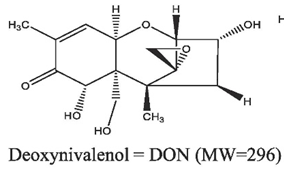
\includegraphics[width=0.25\textwidth]{img/fig_1.png}
    \caption{Formule semi développée du Deoxynivalenol, molécule de la famille des B-trichothécènes produite par les \textit{Fusarium}\cite{gaballah2023development}.}
    \label{fig:mol}
\end{SCfigure}

Jusqu’à présent, le processus de production des mycotoxines a été étudié en ne considérant "qu’un pathogène - une maladie". Cependant, des preuves irréfutables des interactions entre les espèces de \textit{Fusarium} responsables de la fusariose, laisse suggérer que la communication entre ces champignons puisse moduler la régulation de production des toxines.

Afin de mettre en exergue les mécanismes de production de ces molécules inter-individus, il est nécessaire changer d'échelle d'analyse afin d’observer plus globalement le "Meta-Fusarium sp." qui comprend les principales espèces impliquées dans l’infection \cite{ponts2009fusarium, mycsa}. \\

\begin{SCfigure}[1][h]
    \centering
    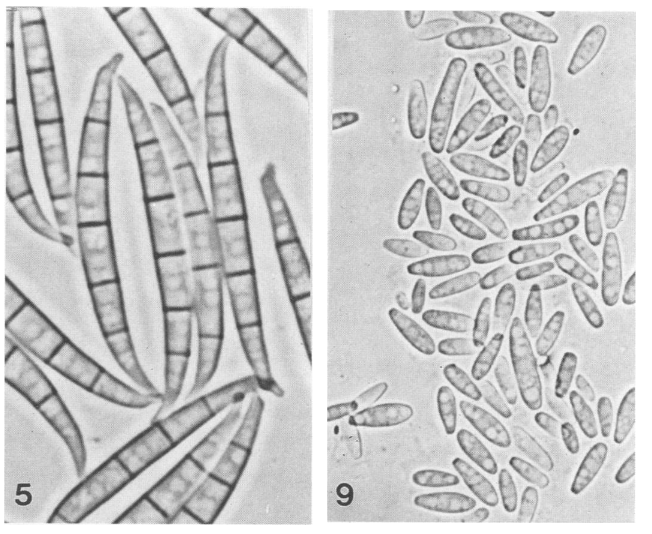
\includegraphics[width=.40\textwidth]{img/fig_2.png}
    \caption{Observation 5 : de macroconidies de \textit{F.graminearum} (950X), 9 : de microcondies de \textit{F.verticillioides} (avant \textit{F.moniliforme} \cite{name}) (1000X) qui sont des champignons qui font partie du Meta-\textit{Fusarium sp} \cite{taxonomy}.}
    \label{fig:fusa}
\end{SCfigure}

\subsection{Communication au sein du Meta-
\textit{Fusarium sp.}}
Au sein du Meta-\textit{Fusarium sp.}. la communication s’effectue en partie par le biais de petits acides ribonucléiques comme les small ARN (smRNA) ou les micro ARN (miRNA). Ces derniers sont des courtes séquences de bases non codantes qui peuvent être séquencées.\\

\begin{figure}[h]
    \centering
    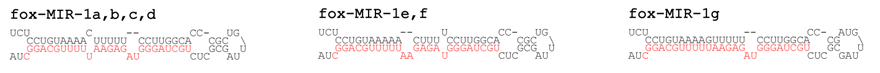
\includegraphics[width=1\textwidth]{img/fig_3.png}
    \caption{Structure secondaire de quelques précurseurs miARN déjà mis en évidence chez les champignons du genre \textit{Fusarium} \cite{chen2014exploring}.}
    \label{fig:mirna}
\end{figure}

Ces petites molécules d'ARN non codantes d'environ 22 nucléotides, sont impliqués dans la régulation post-transcriptionnelle de l'expression génique. En identifiant les miARN spécifiquement produits lors de la communication induite par la rencontre entre deux Fusaria de la même souche, nous pourrons mieux comprendre les mécanismes sous-jacents aux interactions entre les espèces de \textit{Fusarium} toxinogènes. Et ainsi, développer des stratégies de prévention contre la contamination des cultures par les champignons \textit{Fusarium} \cite{ponts2009fusarium, mycsa}.  L’objectif du projet est d’analyser les données séquencées et d’identifier les microARN produits dans chaque scénario de culture, d’en repérer les spécificités et de les quantifier.

\section{État de l'art}
Les pipelines de bio-informatiques visant à gérer des données des séquençages sont très divers et variés. Afin répondre au mieux aux problématiques du client, nous avons réalisé une recherche bibliographique pour rassembler un bouquet d'outils modernes et parfaitement adapté à la tâche. 

L'analyse de données de séquençage de petits ARN dans le contexte de cocultures de céréales et de champignons du genre \textit{Fusarium} nécessite une série d'étapes méthodologiques bien définies. Tout d'abord, l'évaluation de la qualité des données (QC) est essentielle, réalisée grâce à des outils comme FastQC pour obtenir des statistiques détaillées sur la qualité des lectures et MultiQC pour agréger les résultats de plusieurs analyses. Ensuite, le nettoyage des lectures est effectué à l'aide d'outils comme Cutadapt, spécialisé dans l'élimination des adaptateurs, pour préparer les lectures pour l'alignement sur le génome.

L'alignement des lectures sur le génome est une étape cruciale, nécessitant un outil optimisé pour la précision et la gestion des lectures multimappées. BWA-MEM2 est recommandé pour ces raisons. Une fois les lectures alignées, l'identification des petits ARN produits se fait en utilisant ShortStack qui peut annoter ceux déjà connus les ARN connus et isoler les nouveaux, permettant une analyse exhaustive des données. De plus, une indexation des ARN aura lieu grâce à la suite Samtool permettant de gérer les données génomiques de façon très efficace. 

Ces algorithmes se basent sur la recherche de motifs dans des textes grâce à la transformée de Burrows-Wheeler. Elle est à ce jour la méthode algorithmique la plus efficace pour aligner des chaînes de caractères entre elles. 

Le pipeline sera livré sous forme de scripts Python appelant une série de scripts jonglant avec les données.

\section{Présentation des données}

\begin{figure}[ht]
    \centering
    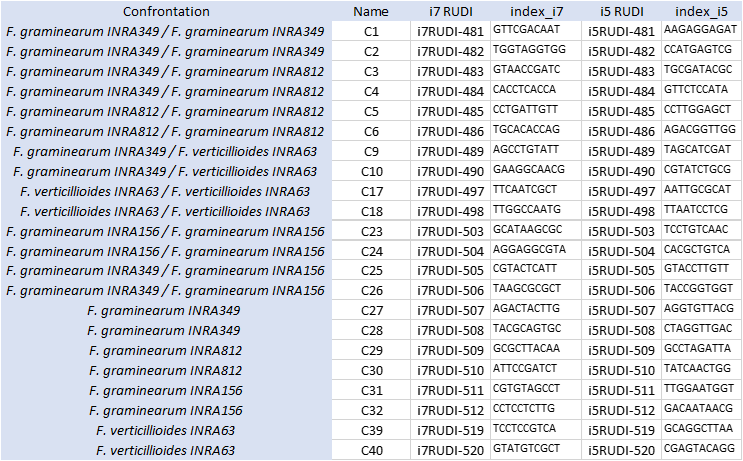
\includegraphics[width=0.8\textwidth]{img/dataset.png}
    \caption{Présentation du jeu de données fourni par le client}
    \label{fig:dataset}
\end{figure}

Pour réaliser ce projet, nous avons travaillé avec un ensemble de données composé de 14 lots en co-culture et 8 lots en mono-culture, comme le montre la figure \ref{fig:dataset}. Ces lots sont des données issues du séquençage Illumina à lecture courte (Short Read), fournies au format FASTQ compressé et désigné par l'extension de fichier ".fastq.gz". Les co-cultures représentent des confrontations entre différentes souches de Fusarium. Les espèces spécifiques utilisées dans cette étude sont Fusarium graminearum, qui comprend les souches INRA349, INRA812 et INRA156, ainsi que Fusarium verticillioides avec la souche INRA63.\\

Chaque lot est identifiée par un nom unique et est associée à des séquences spécifiques, nommées i7 et i5. Ces séquences sont utilisées pour le multiplexage, une technique qui permet d’identifier chaque échantillon de manière unique. Par exemple, la confrontation entre deux souches de F. graminearum INRA349, désignée sous le nom de C1, est associée aux séquences i7 RUDI-481 et i5 RUDI-481.Équipés de données détaillées, nous procédons à l'articulation des besoins spécifiques et des exigences de notre analyse, préparant le terrain pour la conception subséquente de notre pipeline bioinformatique\\


\section{Analyse des besoins}

\subsection{Besoins fonctionnels}
Pour le prétraitement des données, les besoins comprennent :
\begin{itemize}
    \item Acquisition des données issues du séquençage Illumina (Short Read) générées à partir de différentes conditions de culture de Fusarium au format FASTQ.
    \item Prétraitement et nettoyage des données brutes afin d'éliminer les séquences de faible qualité et les erreurs techniques en réalisant un contrôle qualité des lectures.
    \item Normalisation des données.
\end{itemize}

Pour l'analyse des données, les besoins incluent :  
\begin{itemize}
 \item Alignement des lectures prétraitées sur les génomes de référence des souches de Fusarium.
    \item Identifier les miARNs, déterminer leur origine ou leur localisation génomique, et évaluer leur quantité.
    \item Analyse comparative des profils d'expression des microARN entre les échantillons de cultures pures et ceux des confrontations entre souches.
    \item Visualisation des résultats à travers des tableaux et des graphiques codifiés présentant les profils d'expression des miARNs dans les différentes conditions de culture.
\end{itemize}

\subsection{Besoins non fonctionnels}
\begin{itemize}
    \item Utilisation recommandée des langages de programmation adaptés à la bioinformatique, tels que Python, R et éventuellement Bash.
    \item Traitement efficace des données dans des délais raisonnables.
    \item Fiabilité et robustesse pour minimiser les risques de perte de données ou d'erreurs dans l'analyse.
    \item Intuitivité pour une utilisation aisée par les chercheurs non spécialisés en bioinformatique.
    \item Documentation claire et interfaces rationnelles pour faciliter la navigation et l'utilisation des fonctionnalités.
\end{itemize}

\subsection{Contraintes}
\begin{itemize}
    \item Utiliser des outils open source afin d'assurer la transparence, la réutilisabilité du système.
    \item Effectuer nos tâches dans un cadre à accès pseudo-restreint.
    \item Sortir un fichier BigWig compatible avec les plates-formes de navigateur de génome fonctionnelles existantes comme JBrowse pour garantir une visualisation adéquate.
\end{itemize}

\subsection{Ajouts optionnels}
\begin{itemize}
    \item Création d'une base de données pour stocker les résultats.
    \item Sauvegarde et reprise du processus d'analyse et reprise de l'analyse là où elle s'est arrêtée.
    \item Identification des cibles potentielles des miARNs dans les génomes des souches.
\end{itemize}
\chapter{Conception}
Passant du cadre théorique à l'application pratique, cette section décrit la conception et le flux opérationnel de notre pipeline bioinformatique
\section{Flux opérationnel}
Voici un diagramme reprenant les différents points de la conception de notre travail.
\begin{center}
    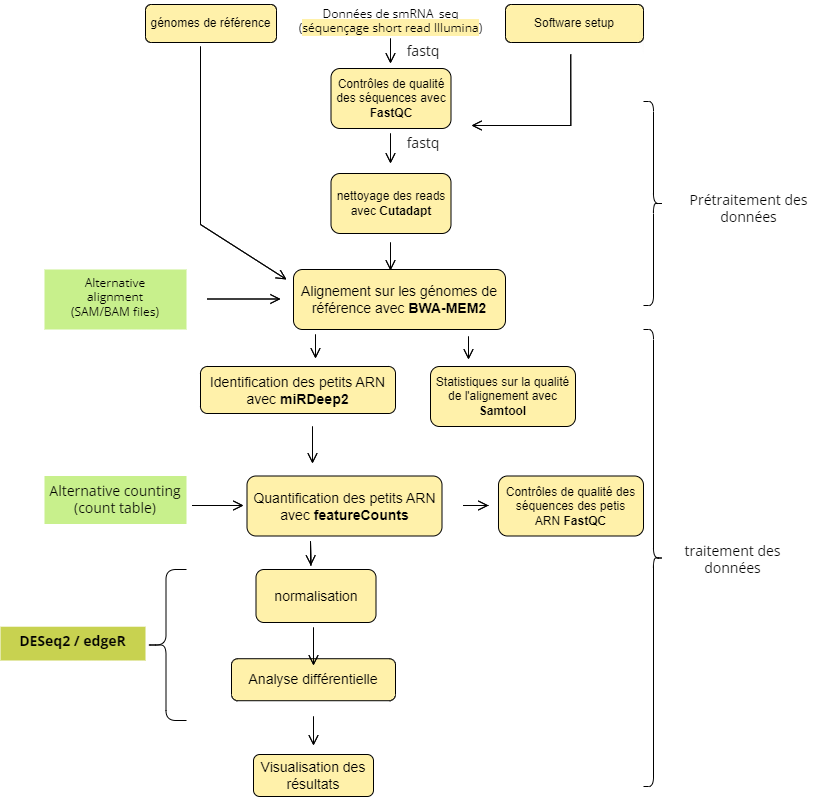
\includegraphics[scale=0.5]{img/PIPLINE_RNA.png}\\[1cm]
\end{center}

\section{Contrôle de qualité}
Les séquences que le client nous a fournis stockées dans des fichiers sont soumises à deux nombreuses erreurs potentielles. Avant d’arriver dans les fichiers, les séquences ont été extraites de matériel vivant, isolées, lavées, préparées, amplifiés, séquencées… la liste est longue. Afin de vérifier qu’au cours de ces étapes précises, le matériel biologique a correctement été transcrit dans les Fastq un contrôle qualité de ces derniers est nécessaire. 

Le contrôle qualité est une étape très classique appliqué sur des séquences de nucléotides. On en extraira de nombreuses métriques qui pourront nous indiquer d’une part si le séquençage s’est bien déroulé mais aussi nous donner des indications de l’anatomie générale des reads que nous avons obtenus. \\

\noindent Parmi les mesures que nous obtiendrons grâce à notre contrôle qualité, nous allons garder un œil sur plusieurs d’entre eux :
\begin{itemize}
    \item  La taille moyenne des reads devrait se rapprocher des tailles des miARN attendus. 
    \item La qualité de lecture des bases devrait être forte car nous somme en short reads. 
    \item De nombreuses séquences d’adaptateurs devrait être présentes dans nos échantillons car ils ont été utilisés pour la préparation des miARN. Leur présence devrait se traduire par un grand nombre de séquences dupliquées. 
\end{itemize}


\section{Nettoyage des reads (trimming)}
Après avoir effectué un contrôle qualité des séquences, il est apparu que plusieurs traitements étaient nécessaires sur les fichiers bruts avant de pouvoir les exploiter. Le trimming représente une étape cruciale car il permet d'éliminer les séquences superflues en vue de nos analyses futures. De plus, certaines parties des reads peuvent avoir été utilisées pour leur indexation, rendant ainsi indispensable leur suppression afin de restaurer un contexte biologique cohérent.


\subsection*{Trimming classique}
Lors de l'utilisation standard d'un outil de filtrage des séquences, nous débutons par la discrimination des lectures de bases de mauvaise qualité. En effet, nos données de séquençage, stockées dans des fichiers FastQ, associent chaque base à un score de qualité Phred. Ce score nous renseigne sur la probabilité que la lecture de la base actuelle soit incorrecte. Ainsi, pour garantir la fiabilité des données, il est nécessaire d'éliminer toutes les bases présentant une forte probabilité d'erreur \cite{phread}.\\


Les séquençages Illumina présentent une perte de qualité croissante selon la longueur du fragment, attribuable aux méthodes de production. Ainsi, les bases de faible qualité se retrouvent souvent du côté 3’ du brin d'ARN. Pendant le trimming, nous éliminerons les bases en 3’ une par une jusqu'à ce qu'il ne reste plus de bases de faible qualité. Ce processus réduit légèrement la taille moyenne des fragments, mais dans notre cas de séquençage de miARN, ces derniers sont si courts que la qualité n'a pratiquement pas le temps de diminuer.\\

Ensuite, le séquençage Illumina nécessite l'utilisation d'adaptateurs pour fixer les ARN sur la flowcell avant amplification. Bien que ces séquences soient nécessaires, elles doivent être retirées des lectures avant leur étude \cite{illumina}. 

\begin{SCfigure}[1][h]
    \centering
    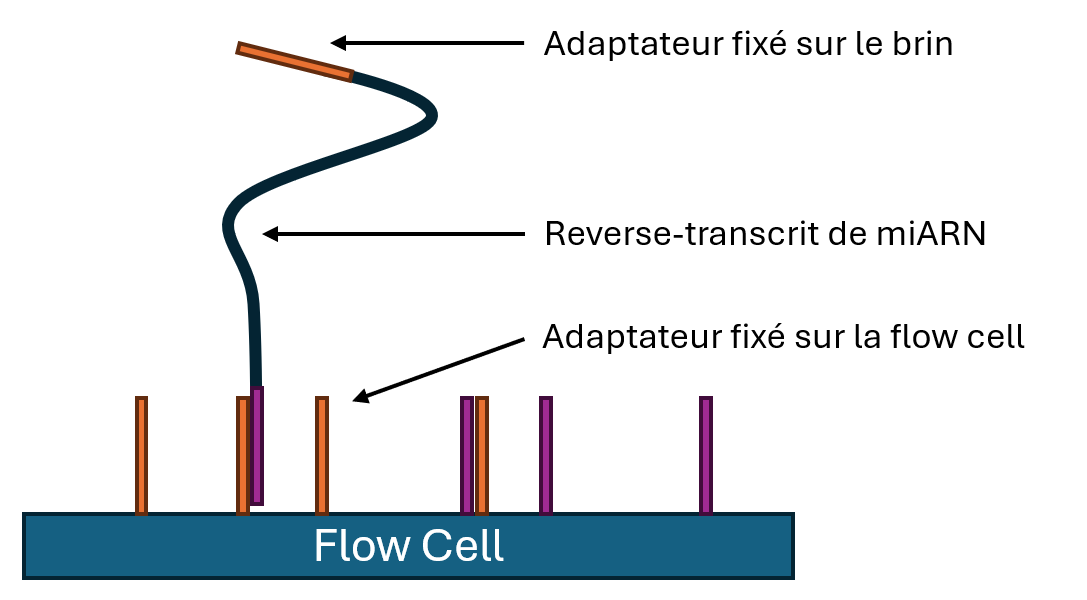
\includegraphics[width=0.5\textwidth]{img/flowcell.PNG}
    \caption{Schéma d'une flowcell fixant un brin d'ADN reverse transcrit à partir d'une séquence de miARN}
    \label{fig:flowcell}
\end{SCfigure}

\subsection*{Trimming additionnel}
\noindent Au-delà des adaptateurs spécifiques à Illumina, nos données contiennent de nombreuses autres séquences qui doivent être supprimées. Voici une liste exhaustive des adaptateurs supplémentaires :

\begin{itemize}
    \item Les \textbf{adaptateurs miRNA} : présents en 5’ et 3’, ils permettent d'améliorer considérablement les séquençages short reads des petits ARN.
    \item Les \textbf{séquences I5 et I7} : elles permettent de différencier plusieurs échantillons dans une même expérience, et sont uniques pour chaque condition expérimentale, étant présentes en 5’ et 3’.
    \item Enfin, avant l'adaptateur Illumina, une \textbf{UDI (Unique Dual Index)} est présente en 3’, permettant le multiplexage entre différentes expériences. Cela permet d'optimiser les ressources en introduisant une grande quantité de matériel génétique dans le séquenceur.
\end{itemize}

\begin{figure}[ht]
    \centering
    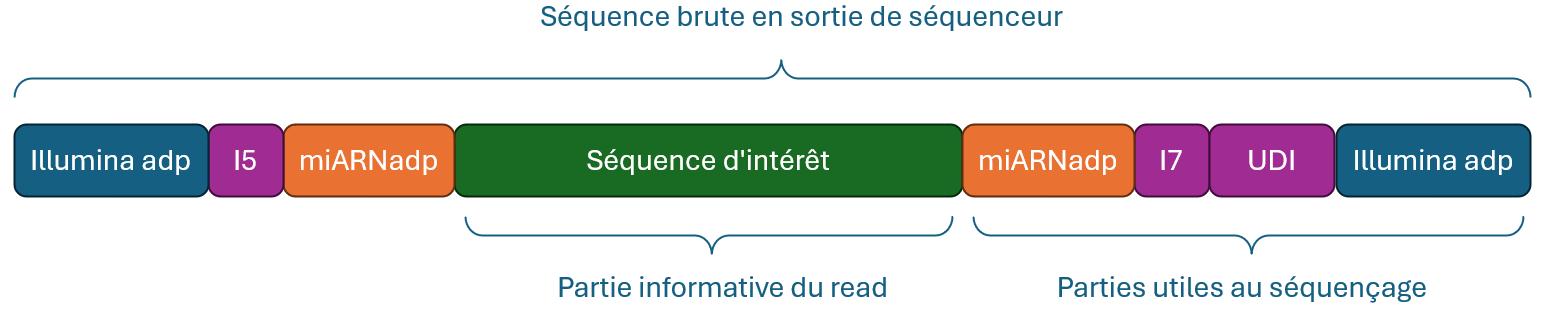
\includegraphics[width=1\textwidth]{img/sequence.PNG}
    \caption{Diagramme illustrant la composition des séquences brutes.}
    \label{fig:sequence}
\end{figure}

Notre code est confronté à un défi majeur : les séquences I7 et I5, qui permettent de différencier les échantillons, sont uniques pour chaque condition expérimentale. Par conséquent, nous devons les retirer de manière dynamique. Pour gérer cette problématique, nous avons créé un fichier CSV (valeurs séparées par des virgules) qui servira de base de données pour sélectionner les différentes séquences à retirer. Les séquences I7/5 concernées seront intégrées à l'outil aux côtés des adaptateurs Illumina, des miARN et de l'UDI.\\

\section{Alignement des séquences}
Une fois nos séquences nettoyées, nous allons les aligner sur leurs génomes de référence afin de caractériser leurs emplacements. Cette étape est cruciale car elle permettra d’avoir une visualisation plus globale de nos données. 

Deux complications nous font faces pour cet alignement. Tout d’abord la nature même de nos séquences rend difficile leur localisation, les reads de miARN font environ 22 nucléotides de long ce qui laisse place à des erreurs d’alignement notamment sur les zones conservées de ces derniers.

D’autre part, nous avons des échantillons qui sont mesurées dans des situations de coculture. Quand la coculture est effectuée entre différente souches, il faudra être capable d’aligner sur plusieurs génomes de références. 

\section{Identification des miARN}
Grace a l’alignement, des séquences, une identification des miARN sera possible. Cette dernière marquera le dernier traitement sur les données que nous effectuerons. Elle permettra d’apprécier les types de miARN produits et leurs quantités dans chaque zone du génome. Nous regarderons notamment la quantité d’ARN ribosomique ainsi que la position des reads au sein des régions non codantes. 

Cette identification nous permettra d’observer si la variabilité au sein de cette population de miARN est forte ou s’ils sont dominés par des groupes bien définis. Mais surtout nous pourrons comparer quantitativement les scénarios de coculture et de monoculture pour essayer d’identifier les potentiels ARN qui sont plus produit dans les cas ou deux champignons sont confrontés. 

Après normalisation, si le ratio de différence d’expression d'un ANR entre des conditions expérimentales est élevé, ces derniers seront des cibles de choix pour des études plus poussé sur leurs fonctions propres. 

\section{Le Pipeline}
Le pipeline sera découpé en plusieurs scripts qui jongleront entre eux avec les données. Cette approche permet une modularité accrue, facilite la gestion et la réutilisation du code. Si, dans le futur, le client souhaite adapter le pipeline à deux nouveaux besoin, il lui suffira de modifier un seul script. 
Les résultats d'une étape alimentent la suivante, ainsi, tant que les formats de fichiers sont respectés le programme pourra fonctionner. Cela permet aussi d'utiliser plusieurs langages et prendre le mieux adapté pour chaque étape du pipeline.


\chapter{Réalisation}
S'appuyant sur un pipeline bien conçu et minutieusement vérifié, la phase de réalisation implique le traitement effectif des données, passant de la théorie à la pratique
\section{Contrôle de qualité}

Avant de procéder à toute analyse, nous avons effectué un contrôle qualité des séquences à l'aide de l'outil FastQC. Cette étape est essentielle pour évaluer la qualité des données brutes et identifier d'éventuels problèmes ou biais qui pourraient affecter les résultats de nos analyses ultérieures.

\subsection*{L'outil}

FastQC est un outil facile à utiliser qui accepte les fichiers de données brutes en format FastQ. Il génère un rapport HTML interactif qui peut être visualisé dans n'importe quel navigateur web. Ce rapport contient une série de graphiques et de tableaux qui aident à comprendre la qualité des données de séquençage \cite{fastqc, fastQC2}.\\

FastQC et à travers son rapport généré, nous permettent d'examiner différentes métriques de qualité, telles que la distribution des scores de qualité, la présence de séquences dupliquées, la présence d'adaptateurs, la qualité de base par position, etc. En examinant ces métriques, nous pouvons déterminer si les données répondent aux critères de qualité requis pour nos analyses et si des étapes supplémentaires, telles que le trimming, sont nécessaires.\\

L'interprétation des résultats de FastQC nécessite une certaine expertise. Chaque module du rapport fournit une "passe" ou un "échec" basé sur les seuils définis pour les données de séquençage de haute qualité. Cependant, un "échec" dans un module ne signifie pas nécessairement que les données sont de mauvaise qualité. Il est important de comprendre le contexte biologique et l'objectif de l'expérience pour interpréter correctement ces résultats.

\subsection*{Le Bloc de commandes}
Ce script, écrit en Bash, automatise l'évaluation de la qualité des données de séquençage en utilisant FastQC. Il est conçu pour améliorer l'efficacité des pipelines bioinformatiques, le script prend deux arguments en entrée : le répertoire d’entrée contenant les fichiers .fastq.gz et le répertoire de sortie où les résultats de l’analyse seront stockés. Si le répertoire de sortie n’existe pas, le script le crée. Ensuite, il utilise la commande find pour rechercher tous les fichiers .fastq.gz dans le répertoire d’entrée. Pour chaque fichier trouvé, il exécute l’outil FastQC, qui analyse la qualité des séquences. Les résultats de l’analyse FastQC sont ensuite enregistrés dans le répertoire de sortie.\\

Après avoir analysé les résultats de FastQC, nous avons identifié plusieurs aspects nécessitant une attention particulière, notamment la présence d'adaptateurs, qui pourraient affecter la fiabilité des données. Ces séquences d'adaptateurs peuvent être éliminées à l'aide d'outils de trimming tels que Cutadapt. Le processus de nettoyage des données va permettre de préparer les données pour les analyses ultérieures.\\

\section{Nettoyage des reads}
Cutadapt représente un outil performant dédié au nettoyage des séquences, capable de filtrer les données selon de multiples paramètres. Fondé sur la transformée de Burrows-Wheeler, il permet une recherche hors ligne de motifs dans un texte. Plusieurs outils sont disponibles pour le trimming des séquences, et nous avons opté pour Cutadapt en raison de sa spécialisation dans le retrait des adaptateurs \cite{martin2011cutadapt}. 

\subsection*{Les métriques de longueur et qualité}
L'outil Cutadapt accepte en paramètre des longueurs maximales et minimales de lectures. Ces paramètres permettent d'exclure toutes les séquences qui ne répondent pas aux normes des miARN. Ainsi, notre longueur maximale est fixée à 30 nucléotides et notre longueur minimale à 15 nucléotides. De cette manière, nous ne conservons que les séquences qui peuvent potentiellement nous être utiles.

\subsection*{L'automatisation}
Le script qui gère l'exécution de cet outil est écrit en Bash. Tout d'abord, il appelle les différents fichiers d'entrée et de sortie des données, ainsi que le fichier CSV contenant les séquences I7/5. Pour permettre à l'utilisateur d'injecter ses propres séquences et éviter les éventuels problèmes et exécutions inutiles, une vérification préalable à l'exécution du trim est effectuée pour garantir que les séquences I7/5 sont conformes aux normes IUPAC. Ensuite, le fichier des données fastaQ est temporairement décompressé avant d'être injecté dans Cutadapt. Pendant tout le traitement, les opérations réalisées par le script sont affichées dans le terminal pour fournir un retour d'information à l'opérateur.

\section{Alignement des séquences}

\subsection*{Accélérer le traitement}
L’alignement des reads sur un génome est une opération a lourde charge computationnelle. Elle implique la recherche de motif (les reads) dans un texte très long (le génome). \\

\noindent BWA\_MEM2 est un algorithme qui associe toutes les techniques les plus modernes pour réduire au maximum le temps de calcul. Voici une liste non exhaustive des « astuces » utilisées ici : 

\begin{itemize}
    \item L’utilisations de la transformée de Burrow Wheeler, cité plusieurs fois dans ce rapport, permet de fortement compresser le texte en regroupant les motifs de ce dernier. 
    \item L’implémentation du parallélisme, il fait référence à la capacité d'exécuter simultanément plusieurs tâches ou instructions en utilisant plusieurs cœurs de processeur sur une même machine. En répartissant la charge de travail les opérations sont réalisées plus rapidement et efficacement.
    \item L’amélioration principale de BWA\_MEM2 sur son prédécesseur BWA est l’implémentation d’une phase de « seeding ». Elle implique d'identifier de courtes correspondances exactes entre un read et le génome de référence. Ces correspondances exactes servent de points de départ pour le processus d'alignement. L'objectif de la phase de « seeding » est d'identifier rapidement des régions potentielles d'alignement, réduisant ainsi l'espace de recherche et la complexité computationnelle des étapes d'alignement suivantes \cite{LISA, MEM2Github}.
\end{itemize} \\ 

\noindent Grace à ces optimisations, cet algorithme est environ deux fois plus rapide que son prédécesseur \cite{bwamem2, BWAimproved}.

\subsection*{La séquence de commandes}
Pour cet outil aussi, le script est écrit en bash, le shell permet une grande simplification du script. Un fichier JSON contenant les accès aux différents fichiers d’input/output est appelé puis les différents génomes de référence sont importés. 

\subsubsection*{L’indexation}
Les index (dans le cadre de l’alignement) sont des prétraitements du texte qui permettent de localiser ultérieurement les reads en son sein. Ces index dans le cadre de BWA\_MEM2 sont la transformée de Burrows-Wheeler, la liste des suffixes ou encore l’index de Ferragina-Manzini (compression de la Burrows-Wheeler).

Ce genre de prétraitement est important dans le cas des méthodes dites « offlines » d’alignement, ces méthodes « offlines » prétraitent le texte à l’inverse des méthodes dites « online » qui prétraitent le pattern. Ici, nous avons des millions de patterns (reads) et seulement quelques textes (génomes de référence) nous pouvons ainsi capitaliser les méthodes offlines pour faciliter les calculs. 

Il se trouve que la génération des indexes peut-être plutôt demandante en ressource. Ainsi dans notre script, elle sera appliquée si et seulement si le génome n’est pas déjà annoté. 
Une fois le génome traité si besoin, tous les reads sont alignés un par un et exportés dans un fichier SAM.
 
\section{Génération des index}

% par la suite Samtools

\begin{quote}
    /TO DO/
\end{quote}

% On parle des outils, comment on a implémenté le script et des potentiels problèmes que l'on a eus. On peut aussi donner un exemple de résultat. 

\section{Identification des miARN}

%  avec ShortStack

\begin{quote}
    /TO DO/
\end{quote}

% On parle des outils, comment on a implémenté le script et des potentiels problèmes que l'on a eus. On peut aussi donner un exemple de résultat. 

\section{Fonctionnalitées du pipeline}
\subsection{Le programme de management}

Le programme \texttt{manager.py} est un gestionnaire de scripts conçu pour faciliter l'exécution de différents fichiers Bash dans le cadre d'une analyse de séquençage ARN. Ce gestionnaire est écrit en Python et utilise le module de logging pour enregistrer les étapes de son exécution, assurant ainsi une traçabilité et une transparence lors de l'analyse des données.\newline

L'une des principales fonctionnalités du gestionnaire est sa capacité à charger et valider un fichier de configuration au format JSON, nommé \texttt{rna\_seq\_config.json}. Ce fichier contient des informations sur les programmes disponibles, leurs chemins d'accès et les ordres dans lesquels ils doivent être exécutés. Le script garantit que les configurations nécessaires sont présentes et valides avant d'exécuter les scripts.\newline

Une fois la configuration chargée et validée, le gestionnaire affiche un menu interactif permettant à l'utilisateur de choisir le script à exécuter. Chaque script est accompagné d'une brève description pour aider l'utilisateur à faire son choix. Le gestionnaire prend également en charge la saisie d'arguments supplémentaires pour certains scripts, ce qui lui confère une flexibilité supplémentaire dans son utilisation.\newline

Lors de l'exécution d'un script, le gestionnaire utilise le module \texttt{subprocess} pour appeler le script Bash correspondant avec les arguments appropriés. Les résultats de chaque exécution sont enregistrés à l'aide du module de logging, permettant à l'utilisateur de suivre le déroulement de l'analyse et de détecter rapidement toute erreur ou problème éventuel.\newline

En cas d'erreur pendant l'exécution du gestionnaire lui-même, toutes les exceptions sont capturées et enregistrées à l'aide du logging, assurant ainsi une gestion robuste des erreurs et une meilleure expérience utilisateur.\newline

En résumé, le script \texttt{manager.py} offre une interface conviviale et robuste pour gérer l'exécution de fichiers Bash dans le cadre d'une analyse de séquençage ARN. Grâce à son utilisation du logging et à sa gestion des exceptions, il garantit une exécution fluide et transparente des scripts, facilitant ainsi le processus d'analyse et de traitement des données.


\subsection{L'utilisation du fichier JSON}
Dans notre programme, nous avons fait le choix d’utiliser un fichier JSON. Il est organisé en un format de données léger et lisible utilisé pour structurer des données. Il facilite l’échange d’informations entre des applications. Son utilité réside dans sa simplicité et sa flexibilité, car il permet de représenter des données structurées de manière hiérarchique à l'aide de paires clé-valeur comme un dictionnaire.

Les fichiers JSON sont largement utilisés pour le stockage de configuration, ainsi, dans notre programme il stocke les paramètres des différents scripts ainsi que leur nom et leur rôle.

\begin{SCfigure}[1][h]
    \centering
    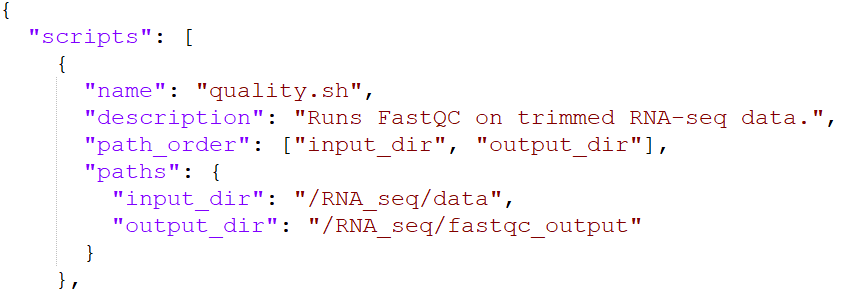
\includegraphics[width=.5\textwidth]{img/exemple_json.PNG}
    \caption{Voici un exemple d’entrée dans notre fichier JSON qui servira à la configuration des scripts.}
    \label{fig:JSON}
\end{SCfigure}


Comme ce format est lisible, il peut facilement être modifié par l’utilisateur et il assure que tous les modules de notre pipeline reçoivent les mêmes informations.


\subsection{Le Logging}

Le logging est une composante cruciale de tout programme informatique, fournissant une traçabilité de l'exécution du programme et facilitant la détection et la résolution des problèmes. Dans le contexte du développement d'une application Python pour l'exécution de commandes Bash, le logging a été intégré de manière à assurer la transparence de l'exécution du programme.\newline

La configuration du logging est définie au début du script, spécifiant le niveau de logging sur INFO et le format des messages. Par exemple, voici une configuration de logging typique :

\begin{lstlisting}[language=Python, breaklines=true]
logging.basicConfig(level=logging.INFO, format='%(asctime)s - %(levelname)s - %(message)s')
\end{lstlisting}

Dans le script fourni, le logging est utilisé pour enregistrer des messages d'importance INFO et supérieure, fournissant ainsi une vue détaillée du déroulement du programme. Par exemple, des messages INFO sont utilisés pour signaler le démarrage et la fin de l'exécution des scripts, ainsi que pour afficher les arguments utilisés lors de l'exécution. Voici un exemple de message INFO enregistré pendant l'exécution du script :

\begin{lstlisting}[language=Python, breaklines=true]
2024-05-12 15:30:00 - INFO - Running script: /path/to/script.sh with arguments: [arg1, arg2, arg3]
\end{lstlisting}

En outre, le logging est également utilisé pour enregistrer les erreurs survenues pendant l'exécution du programme. Les messages d'erreur sont enregistrés avec un niveau de journalisation ERROR, permettant ainsi de les identifier facilement parmi les messages d'état normaux. Par exemple, voici un exemple de message d'erreur enregistré lorsqu'une erreur se produit pendant l'exécution d'un script :

\begin{lstlisting}[language=Python, breaklines=true]
2024-05-12 15:35:00 - ERROR - Failed to execute /path/to/script.sh: Return code 1
\end{lstlisting}

Enfin, le logging est utilisé pour signaler des situations potentiellement problématiques qui ne sont pas des erreurs graves. Ces messages sont enregistrés avec un niveau de journalisation WARNING. Par exemple, voici un exemple de message WARNING enregistré lorsque l'utilisateur saisit une entrée invalide lors du choix d'un script à exécuter :

\begin{lstlisting}[language=Python, breaklines=true]
2024-05-12 15:40:00 - WARNING - Invalid choice, please choose a number between 1 and 4
\end{lstlisting}

L'ensemble de ces messages de logging fournit une traçabilité complète de l'exécution du programme, facilitant ainsi la détection et la résolution des problèmes éventuels. En enregistrant les messages dans un format structuré, il devient également plus facile d'analyser les journaux et d'extraire des informations importantes sur le fonctionnement du programme.

\section{Le fichier ReadMe}

% must add a line or two about ReadMe

\section{Utilisation de Git}

Pour faciliter notre travail collaboratif et assurer une gestion efficace de notre code source, nous avons opté pour l'utilisation de GitHub comme plateforme principale. Les fonctionnalités de contrôle de version de Git ont permis aux membres de l’équipe de travailler ensemble et de suivre les modifications apportées au code tout au long du projet. L'ensemble des scripts, ainsi que le cahier des charges et le rapport en format TeX, ont été déposés dans le répertoire GitHub dédié au projet (https://github.com/Lucien-Piat/RNA-Seq-Fusarium). De plus, GitHub offre à l'ensemble de l'équipe et aux clients un accès pratique et sécurisé au code. En accordant aux clients l'accès au dépôt, ils peuvent non seulement exécuter le programme, mais également examiner le code source lui-même à tout moment.

\chapter{Résultats et Discussion}
\section{Exemple de résultats}
\begin{quote}
    /TO DO/ Ici ajouter les résultats brutes pour illustrer le pipeline
\end{quote}

\section{Discussion}
\begin{quote}
    /TO DO/ Ici discuter rapidement des résultats
\end{quote}

\section{Perspectives}
\begin{quote}
    /TO DO/ Ici décrire rapidement les choses qui pourrait êtres faites dans le futur
\end{quote}

\chapter*{Conclusion}
\addcontentsline{toc}{chapter}{Conclusion}

% à adapter

En conclusion, ce projet a permis de mettre en place un pipeline d'analyse de données RNA-Seq pour étudier l'expression des gènes dans le contexte de cocultures de céréales et de champignons du genre Fusarium. À travers les différentes étapes du pipeline, depuis le prétraitement des données jusqu'à l'analyse en aval, nous avons pu obtenir des résultats précis et significatifs.\newline
    
La première étape du pipeline, l'évaluation de la qualité des données, est réalisée avec précision grâce à des outils tels que FastQC et MultiQC, fournissant ainsi des statistiques détaillées sur la qualité des lectures. Ensuite, le nettoyage des lectures est effectué avec Cutadapt, spécialisé dans l'élimination des adaptateurs, afin de préparer les lectures pour l'alignement sur le génome.\newline
    
L'alignement des lectures sur le génome, réalisé avec BWA-MEM2, constitue une étape cruciale pour obtenir des résultats précis. L'utilisation de ShortStack permet ensuite l'identification exhaustive des petits ARN produits, y compris ceux déjà connus et les nouveaux, facilitant ainsi une analyse approfondie des données. De plus, l'indexation des ARN avec la suite Samtools assure une gestion efficace des données génomiques.\newline
    
Le choix de ces algorithmes, basés sur la transformée de Burrows-Wheeler, s'avère être la méthode la plus efficace pour aligner des chaînes de caractères entre elles, garantissant ainsi la fiabilité des résultats obtenus.\newline
    
Enfin, le pipeline est livré sous forme de scripts Python puis d'un manuel d'utilisation, offrant ainsi une flexibilité et une facilité d'utilisation pour l'utilisateur final, tout en assurant une manipulation efficace des données.\newline
    
En somme, ce pipeline sur mesure répond aux exigences spécifiques de l'analyse de données de séquençage de petits ARN dans le contexte des cocultures de céréales et de champignons du genre Fusarium, offrant ainsi une solution complète et fiable pour les besoins du client.


\bibliography{biblio}

\appendix
\chapter*{Annexes}
\addcontentsline{toc}{chapter}{Annexes}

\section*{Diagramme de Gantt}

\begin{figure}[ht]
    \centering
    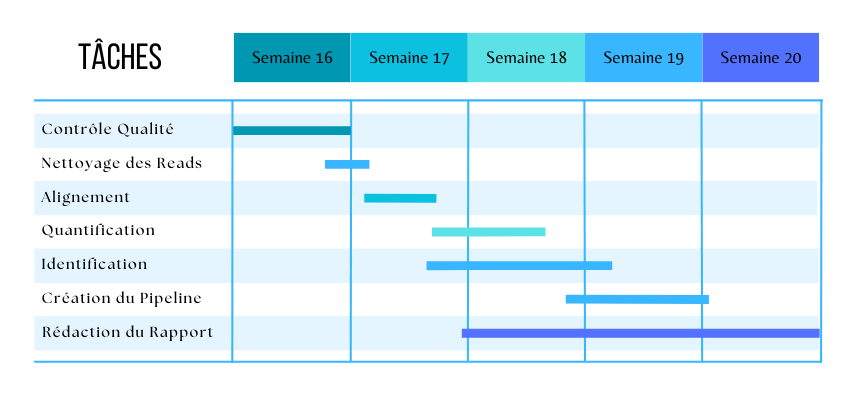
\includegraphics[width=1\textwidth]{img/gantt.png}
    \caption{Diagramme de Gantt qui nous servira de base pour l'organisation de notre travail}
    \label{fig:gantt}
\end{figure} 
\end{document}
